% Emacs, this is -*-latex-*-

% Chunk Flooding

\label{sec:chunk_flooding}

\begin{comment}
\begin{figure*}
  %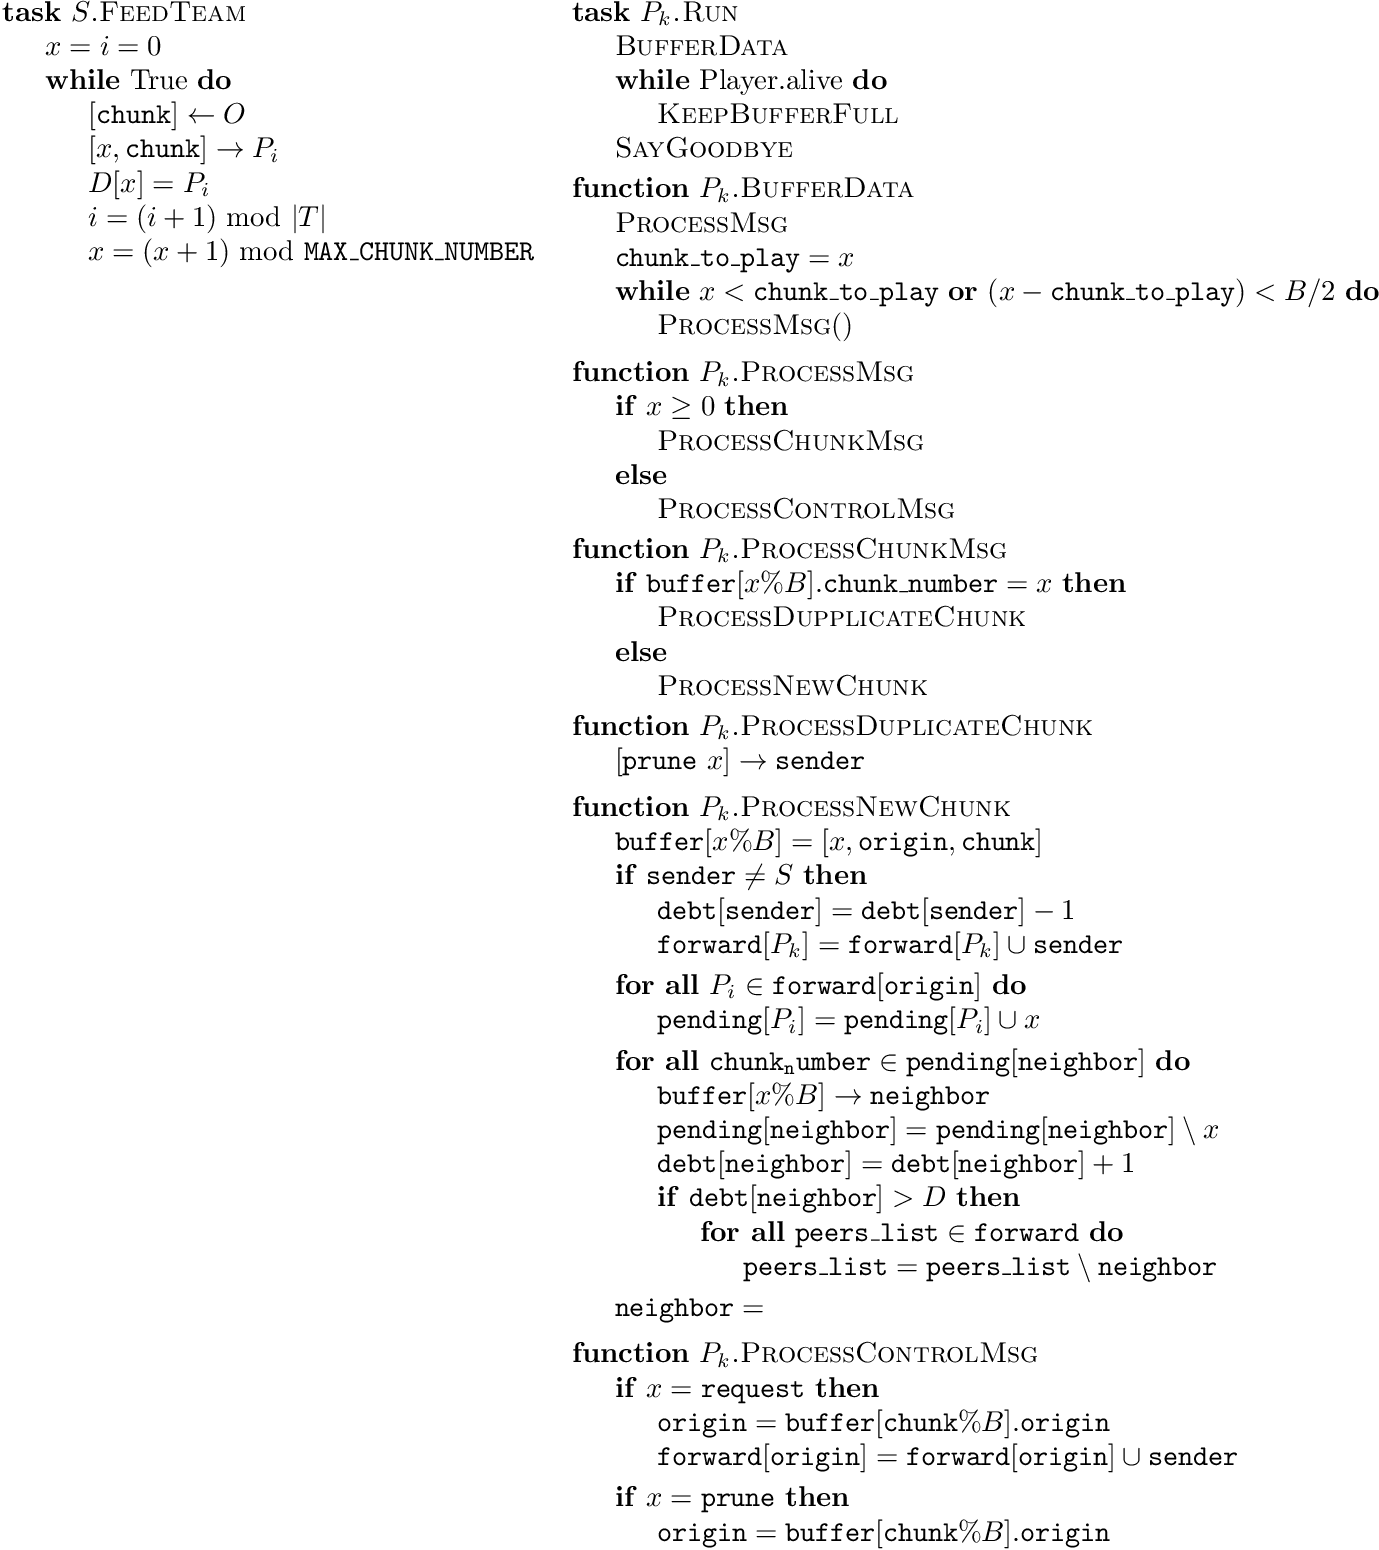
\includegraphics[width=0.75\textwidth]{chunk_generation_and_flooding}
  \imgw{300}{graphics/peer_chunk_flooding.svg}
  \caption{Chunk flooding at peers.\label{fig:peer_chunk_flooding}}
\end{figure*}
\end{comment}

DBS is a push-based protocol. When a peer receives a chunk, it can be
retransmitted to a large number of neighbors,depending on the number
of peers in its forwarding table. Therefore, even if the chunk rate is
controlled by the streaming servers, some kind of flow control must be
performed by the peers in order to reduce network congestion while the
overlay is flooded.

%Moreover, to achieve an ideal I/O ratio of $1$, peers should send one
%chunk for every received one.

The congestion (basically due to the use of the physical link by DBS)
may be avoided following the next idea: \textit{only if I have
  received a chunk, I send (not necessary to the sender) a chunk (not
  necessary the received chunk)}. In a fully connected overlay (see
Fig.~\ref{fig:full_mesh}), this allows to control the data
flow. However, in more realistic scenarios, where the physical media
imposes interconnection constraints (such as those generated by
firewalls and symmetric NATS), peers can not be directly ``connected''
with the rest the team. Therefore, if the splitter follows a pure
round-robin strategy, some peers will send more chunks than they
receive in order to flood the overlay (as happens for example in
Fig.~\ref{fig:star}). In these scenarios, the simple idea of sending a
chunk for each received one does not work.

Fortunately, the previous idea can be adapted to handle a variable
connectivity degree (also called \gls{neighborhood-degree}).  Each
peer uses a table of lists, $\mathtt{pending}[]$, indexed by the
neighbor's end-points, where each list references the positions in the
buffer of those chunks in the current peer that must be transmitted to
the corresponding neighbor the next time such neighbor is selected in
the flooding process. For example, if
$\mathtt{pending}[P_x]=\{11,22\}$, chunks found at positions $11$ and
$22$ of the buffer have to be sent to peer $P_x$.

Notice that using this procedure, more than one chunk can be sent to a
neighbor in a transmission burst. This could congest the physical
devices in very unbalanced overlays (see the
Fig.~\ref{fig:star}). Therefore, on average short bursts are
desired. As an advantage, all the chunks of the burst travel between
the two same hosts when a burst is produced, which usually increases
the performance of the layer-3 routing. Additionally, those chunks
could be grouped in one single packet, reducing the protocol overhead.

An example of the temporal evolution of a team using the flooding
algorithm has been described in the Figures \ref{fig:team_0} to
\ref{fig:team_4}. \leorem{Mejor usar captions pequeños ($t_0$ y $t_1$) y
  describir en el texto, usar subfiguras}.

\begin{figure}
  \myfig{graphics/team_0}{5cm}{250} %
  \caption{A team has been created with a single monitor $M_0$
    ($[\mathtt{hello}]$ messages are not shown). Chunks with numbers 0
    and 1 (the time $t$ is measured in chunks-time) have been
    transmitted from the splitter $S$ to $M_0$. $f$ and $p$ represents
    the $\text{forward}[]$ and the $\text{pending}[]$ structures,
    respectively. The chunks stored in the buffer are shown below the
    entity.} %
  \label{fig:team_0}
\end{figure}

\begin{figure}
  \myfig{graphics/team_1}{5cm}{250} %
  \caption{At $t_2$, peer $P_1$ joins the team (the
    $[\mathtt{hello}]$'s are not shown). In $M_0$, $f=\{M_0:[P_1]\}$
    because when $M_0$ receives the $[\mathtt{hello}]$ from $P_1$,
    $M_0$ is the origin peer for all chunks received from $S$ and
    $P_1$ is its neighbor. $P_1$ includes an entry $P_1:[M_0]$ in its
    forwarding table because $M_0$ is in the set of peers received
    from the splitter. After that, when the chunk number 2 arrives to
    $M_0$ from $S$, an entry $P_1:2$ is created in $p$ for that
    chunk, and this entry is deleted when the chunk 2 is sent to
    $P_1$.} %
  \label{fig:team_1}
\end{figure}

\begin{figure}
  \myfig{graphics/team_2}{6cm}{250} %
  \caption{$P_2$ joins the team. $M_0$ and $P_1$ includes $P_2$ in
    their forwarding tables. The chunk 3 is received by $P_1$ which
    decides to send it to $P_2$. Chunk 3 remains as pending to be sent
    to $M_0$ when the next chunk is received by
    $P_1$.} %
  \label{fig:team_2}
\end{figure}
%  $P_2$ is the origin peer for $M_0$ and $P_1$ because both of them are in the list of peers that $P_2$ receives from $S$.
    
\begin{figure}
  \myfig{graphics/team_3}{6cm}{250} %
  \caption{Chunk 4 is received by $P_2$ which relays it to $P_1$, what
    relays chunk 3 to $M_0$.} %
  \label{fig:team_3}
\end{figure}

\begin{figure}
  \myfig{graphics/team_4}{6cm}{250} %
  \caption{Chunk 5 is received by $M_0$ which
    relays it to $P_2$.} %
  \label{fig:team_4}
\end{figure}

\begin{notex}
  \begin{figure*}
    \myfig{graphics/team_5}{4cm}{350}
  \end{figure*}
  
  \begin{figure*}
    \myfig{graphics/team_6}{4cm}{380}
  \end{figure*}
  
  \begin{figure*}
    \myfig{graphics/team_7}{4cm}{320}
  \end{figure*}
  
  \begin{figure*}
    \myfig{graphics/team_8}{4cm}{200}
  \end{figure*}
  
  \begin{figure*}
    \myfig{graphics/team_9}{4cm}{280}
  \end{figure*}
  
  \begin{figure*}
    \myfig{graphics/team_10}{4cm}{380}
  \end{figure*}
  
  \begin{figure*}
    \myfig{graphics/team_11}{4cm}{210}
  \end{figure*}
  
  \begin{figure*}
    \myfig{graphics/team_12}{4cm}{210}
  \end{figure*}
  
  \begin{figure*}
    \myfig{graphics/team_13}{4cm}{210}
  \end{figure*}

\end{notex}

%An example of the flooding with congestion control algorithm has been
%show in the Figs.~\ref{fig:team_0}, ...
%Notice that in this example
%all messages are received successfully.
%As can be seen in the example, when a peer $P_k$ receives a chunk,
%$P_k$ floods a number of chunks to one of its its neighbors (obviously,
%except the neighbor sender of the chunk), using round-robin
%schema. The size of this set, what we call $\text{pending}$, depends
%on how many neighbors a peer has.

% Alternative: increment by +1 and decrement by /2

% Alternative: peers keep sorted the neighbors by debt, and the list
% is run from the beginning each time a chunk arrives from the
% splitter.

% Alternative: the debt is only incremented if the relayed chunk has
% been received from the splitter.

% Alternative: if between two consecutive chunks received from the
% splitter (a round), a peer does not receive a chunk from a neighbor
% with origin such neighbor, the peer is removed from the forwaring
% list.

\begin{comment}
In each round, peers check if a chunk have been received from the rest
of peers of the team (${\cal P}_k\in {\cal T}_j)$). If not, peers send
a $[\mathtt{propagate}~{\cal P}_i]$ to one or more (possibly
to the rest of) peers of the team, where ${\cal P}_i$ is the origin peer
of the missing chunk. At this point, the process continues as
described in Section~\ref{dbs:chunk_flooding}.
\end{comment}

\begin{comment}
For each ${\cal P}_k\in N({\cal P}_i)$, ${\cal P}_i$ checks if a chunk
has been received from ${\cal P}_k$. If ${\cal P}_i$ detects that
${\cal P}_k$ has not sent a chunk to it during $L$ consecutive rounds,
performs $N({\cal P}_i) = N({\cal P}_i)\setminus{\cal P}_k$, and stops
sending to ${\cal P}_k$ more chunks.
\end{comment}
\begin{comment}
computes a
``chunk-debt'', denoted by $d({\cal P}_k)$, that is incremented each
time a chunk is received from ${\cal P}_k$ and decremented each time a
chunk is sent to ${\cal P}_k$. If ${\cal P}_i$ verifies that $d({\cal
  P}_k)>D$ (the maximum debt), then ${\cal P}_i$ considers that ${\cal
  P}_k$ is unable to communicate with it, performs $N({\cal P}_i) =
N({\cal P}_i)\setminus{\cal P}_k$, and stops sending to ${\cal P}_k$
more chunks.
\end{comment}

%When peers receive chunks from their splitter, they must flood them to
%their neighbors until the chunks are broadcasted to the whole team
%(Fig.~\ref{fig:chunk_generation_and_flooding}). Lets suppose that
%${\cal P}_k$ receives a chunk. In the case the sender is its splitter,
%${\cal P}_k$ floods the chunk to $N({\cal P}_k)$. However, if the
%sender is a peer ${\cal P}_m\in N({\cal P}_k)$, ${\cal P}_k$ adds
%${\cal P}_m$ to $N({\cal P}_k)$ if ${\cal P}_m$ is a new neighbor, and
%forwards the chunk to the rest of its neighborhood ${\cal P}_n\in
%N({\cal P}_k)\setminus{\cal P}_m$ if ${\cal P}_k$ is in the shortest
%between ${\cal P}_n$ and the origin peer ${\cal P}_i$ of the relayed
%chunk. This will be true if ${\cal P}_k$ is the gateway of ${\cal
%  P}_n$ to go from ${\cal P}_n$ to ${\cal P}_i$. Therefore, a flooding
%with prunning based on shortest path routing is used.

%Peers do not understand the content, but it is
%known that in order to achieve a I/O ratio of 1, peers should send one
%chunk for every received one, on average. To acomplish this, a ${\cal
%  P}_i$ creates a FIFO queue of chunks for each $N({\cal P}_i)$, and,
%for each received chunk, ${\cal P}_i$ forwards a queued chunk from
%each of these queues.

\begin{comment}
A ${\cal P}_i$ forwards one or more chunks if and only if it has
received a chunk. For each received chunk $c_j$, ${\cal P}_i$: 1)
creates a list $l_{c_j}$ with the contents of $N'({\cal P}_i)$, and 2)
sends $c_j$ to $l_{c_j}[0]$ (the first element), and removes
$l_{c_j}[0]$. For each chunk reception, Step 2) is repeated for all
the previously created lists while they are not exhausted.

A solution is a forwarding algorithm based on the following
idea. Peers manage a list of chunks, where every item is a 2-tuple
($c_k$, $P_l$). The field $c_k$ represents the chunk that must be
flooded (if the node that has delivered the chunk is the splitter,
$c_k$ must be relayed towards all the neighbors, otherwise, $c_k$ must
be sent to all the neighbors except the peer that delivered $c_k$),
and the field $P_l$ the last neighbor to which $c_k$ was sent. For
every chunk received, a new tuple is appended to the list of chunks
and the rest of tuples are updated. The field $c_k$ remains constant
but $P_l$ is replaced by the next peer in the list of neighbors for
every received chunk.
\end{comment}
